% Chapter 2: METHODS

\chapter{Methods} % Main chapter title

\label{methods} % For referencing the chapter elsewhere, use \ref{Chapter1} 

%%----------------------------------------------------------------------------------------
%
%% Define some commands to keep the formatting separated from the content 
%\newcommand{\keyword}[1]{\textbf{#1}}
%\newcommand{\tabhead}[1]{\textbf{#1}}
%\newcommand{\code}[1]{\texttt{#1}}
%\newcommand{\file}[1]{\texttt{\bfseries#1}}
%\newcommand{\option}[1]{\texttt{\itshape#1}}

%----------------------------------------------------------------------------------------
The purpose of this methods section is to give an overview on, first, the data used to develop the software tool and how the data were collected, second, image processing basics, and third, which programming languages, definitions and methods were chosen when developing the tool. This will help the reader to replicate, understand and modify the methods and source code of the tool. 

%----------------------------------------------------------------------------------------
%----------------------------------------------------------------------------------------
\section{Data set}

Our data set consisted of high-throughput time-lapse images of \textit{Arabidopsis thaliana} (Arabidopsis) roots taken by a standard Raspberry Pi V2 camera from 5 experiments with 5-6 roots each containing between 32 and 36 images over a period of at least 5 hours, ie every 10 minutes a photo was taken. 
All experimental parameters remained the same across experiments, except for the applied voltage.
%CUT DUE TO STRICT WORD COUNT
%The images were named after the date and time they were taken; information on the strength of the EF in voltage was captured in each folder containing one experiment data set. 
%All the other parameters except for the applied voltage remain the same (e.g. media, temperature, reservoir size). The specifications are available on request.

It should be noted that these images had already been collected in a previous project, and were not obtained as a part of the work described herein.
% and are not subject but only the basis of the work presented here. 


%----------------------------------------------------------------------------------------
%----------------------------------------------------------------------------------------
\section{Experimental setup}

To better understand the nature of the data, we give a high-level explanation of the experimental setup used for data collection in figure [INSERT REFERENCE HERE].

\begin{figure}[h]
	\centering
	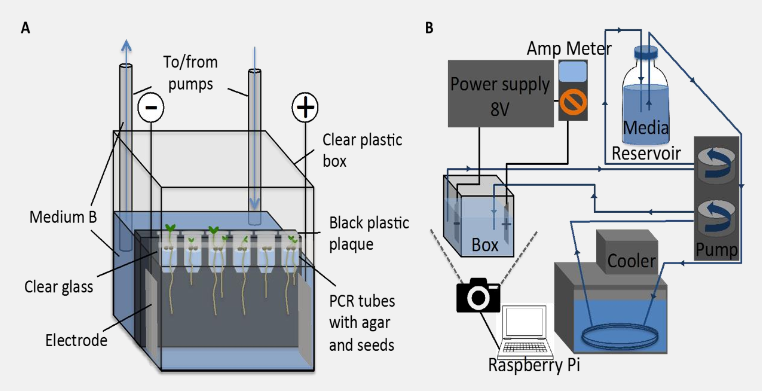
\includegraphics[width=\textwidth]{../Figures/experiment_circuit.png}
	\caption{The experimental setup for root electrotropism: \\
		Subfigure A shows a V-box containing plants in a medium, stabilised by PCR tubes with agar and seedlings. To the left a submerged negative electrode (cathode); to the right a submerged positive electrode (anode); inflow and outflow tube controlling the medium. \\
		Subfigure B shows the components of an EF experiment: The V-box connected to a power source, a media reservoir connected to the V-box via two pumps controlling the medium inflow and outflow, and a camera controlled via a Raspberry Pi facing the V-box to to take time lapse images of the roots at 10 minute intervals. \\
		Taken from [INSERT REFERENCE].}
	\label{fig:experiment}
\end{figure}

[SEE SLIDES, THESIS]

%INSERT FIGURE: PHENOMENOLOGY OF ROOT ELECTROTROPISM]


%----------------------------------------------------------------------------------------
%----------------------------------------------------------------------------------------
\section{Image processing}

Having these images as a basis, the nature of this work was mainly an image processing one.

Image processing pools together a lot of different domains including physics (optics), signal processing and pattern recognition/ Machine Learning (ML); %to ultimately feed computers to understand how to interpret images and make decisions based on them. 
the idea behind it is to extract information from an image in a form that is suitable for computer processing [INSERT REFERENCE HERE]. 

Figure [INSERT REFERENCE HERE] shows fundamental steps in image processing, that served as a guideline for the presented work. However, every single image processing case is different and there will always be slight variations to this generic image processing workflow.


%combines optics and signal processing and is often used in computer vision.
%\begin{enumerate}
%	\item Image aquisition
%	\item Image preprocessing 
%	\item Image segmentation
%	\item Image representation and description -- dep on image that you are studying
%	\item Image understanding
%	\item Results (output)
%\end{enumerate}

[INSERT FLOWCHART FIGURE HERE, adapted from....]


%----------------------------------------------------------------------------------------
\subsection{Digital images}

In image processing, we operate on digital (discrete) images.
An image refers to a 2D light intesity function \( f(x,y) \), where \( (x,y) \) denote spatial coordinates and the value of \( f \) at any point \( (x,y) \) is proportional to the brightness or gray levels of the image at that point [INSERT REFERENCE HERE].
Thus, a digital image is an image \( f(x,y)  \) that has been discretised both in spatial coordinates and brightness, i.e. we

\begin{itemize}
	\item Sample the 2D space on a regular grid
	\item Quantise each sample, i.e. round to nearest integer.
\end{itemize}

What we get is an image represented as a matrix of integer values; the elements of such a digital array are called image elements or pixels.

%If our samples are \( \Delta \) apart, we can write this as:
%\[
%f(x,y) = Quantize{f(\Delta x, \Delta y)}
%\]
%The image can now be represented as a matrix of integer values:

[INSERT EXAMPLE PICTURE HERE]


%----------------------------------------------------------------------------------------
\subsection{On spatial resolution, gray levels and coloured images}

The storage and preprocessing requirements increase rapidly with the spatial resolution and the number of gray levels. 
For instance, a 256 gray-scale image of size 256\( \times \)256 occupies 64K bytes of memory. Figure [INSERT REFERENCE HERE] shows images of different spatial resolution. 

[INSERT FIGURE: Images with decreasing spatial resolution, taken from .....]

Also, an insufficient number of gray levels in smooth areas of a digital image may result in false contouring, see figure [INSERT REFERENCE HERE].

[INSERT FIGURE: Images of different gray-level quantisation]


Since we deal with coloured images, we chose the RGB colour model which is an additative colour model in which red, green and blue light are added together in various ways to reproduce a broad spectrum of colours [INSERT REFERENCE HERE].


%----------------------------------------------------------------------------------------
\subsection{Image processing operations}

An image processing operation typically defines a new image \( g \) in terms of an existing image \( f \).
We can: 
\begin{itemize}
	\item transform the range of \( f \)
	\[ 
	g(x, y) = t(f(x,y)) 
	\]
	\item transform the domain of \( f \)
	\[
	g(x,y) = f(t_{x}(x,y), t_{y}(x,y)).
	\]
\end{itemize}

%IMAGE PROCESSING OPERATIONS USED IN THIS WORK INCLUDE: 

From an image processing point of view, we performed point as well as local operations in our work.

A point operation is a function that is performed on each single pixel of an image, independent of all the other pixels in that image [INSERT REFERENCE HERE]. These include operations like inversing, changing the brightness or contrast of an image, changing the gamma of an image, binarising an image and logical operations. 

Local operations, on the other hand, compute the new value of each single pixel with a neighbourhood around it [INSERT REFERENCE HERE]. %They can be divided in two groups, linear and nonlinear filters.
They include filters which are operations that convert a source image to a result image by applying some kind of tranformation, be it of linear or nonlinear nature [INSERT REFERENCE HERE]. There are more than 134 different filter functions in the MATLAB Image Processing toolbox [INSERT REFERENCE HERE] that can be applied with different arguments and sensitivity thresholds. Filters used in our work include the 2D median filtering \textit{medfilt2} or the 2D adaptive noise-removal filtering \textit{wiener2}.

%A a filter is an operation, which converts a source image via some kind of transformation to a result image [INSERT REFERENCE HERE]. 

% FOR VIIVA: Another possibility for the subdivision of local operations is the division in low-pass and high-pass filters. Low-pass filters are used to inhibit noise and small details on images, whereas high-pass filters are used to emphasize edges."
% http://www.tlmtracker.tu-bs.de/index.php/Image_processing_operations#Threshold


%%%%%%%%%%%%%%%%%%%%%%%%%%%%%%%%%%%%%%%%%%%%%%%%%%----TO DELETE---
%\subsection{Key stages in digital image processing}
%
%[INSERT FLOW CHART HERE]
%
%	Problem Domain -- here plant morphology 
%\begin{itemize}
%	\item Image Aquisition
%	\item Image Enhancement -- contrasting images so human eye can best see things, manipulate values of pixels so you can best caracterise and structure them |
%	\item Morphological Processing -- growing and thinning of pixels, e.g. fingerpringt medical operations
%	\item Image Segmentation -- separating parts of the image such as features and object you want to look at, distribution of pixel values |
%	\item Representation \& Description -- based on quantised space that you're working in. What's realised in that digital output? Two ways to describe features being observed in that pixel space. Inverting etc
%	\item Object Recognition -- see example iris data set. cluster to identify different objects.
%	\item [Computer \& Machine Vision] -- feeds into computer vision and ML
%\end{itemize}
%	[Robotics \& AI], [Deep Learning]
%	
%	feature space that you're working in on top of your labels.
%	put in our own bias and how we train model.
%	
%	A lot of noise in the image makes it grainy. We can apply interpolation, i.e. smoothing the image based on its nn. bi-cubic interpolation.  Smoothes some of the details as well as a side effect, but especially the noise. -- important for edge detection later
%%%%%%%%%%%%%%%%%%%%%%%%%%%%%%%%%%%%%%%%%%%%%%%%%%


%----------------------------------------------------------------------------------------
%----------------------------------------------------------------------------------------
\section{\textit{MATLAB} as a programming language}

As a language we chose \textit{Matlab} as it is very popular in academic circles for image/ data processing given the number of built-in functions, and a well documented image processing toolbox (\textit{MATLAB Image Processing Toolbox} [INSERT REFERENCE HERE]).
%with a very good documentation. 
% GOES TO DISCUSSION/ FUTURE WORK:
%Alternative languages that were considered were \textit{Python} and \textit{Julia}. Another recommended language is \textit{OpenCV} as it is very fast and well documented. Other non-open source software such as \textit{ImageJ}, a Java based image processing program, and \textit{Avizo} which is a general-purpose commercial software application for scientific and industrial data visualisation and analysis with a nice GUI, could not be investigated further in this work. 


%----------------------------------------------------------------------------------------
%----------------------------------------------------------------------------------------
\section{Pre-processing: Getting the root's skeleton}

The goal of the preprocessing step was to extract the skeleton, i.e. the coordinates of the pixels that represent the root on the image.
This task turned out to be highly challenging on noisy image data and can be regarded as the actual achievement of the presented work. The highly elaborate pipeline of the preprocessing step can be found in chapter [INSERT REFERENCE HERE].


% TO DELETE
%For the
%The initial problem of coming up with a "good" definition by comparing different angle and curvature definition shifted. The focus was now on the pre-processing, the extracting the skeleton. 
%However, we will still present some possible definitions of angles and curvature, also not implemented in the current version of the tool.


%----------------------------------------------------------------------------------------
%----------------------------------------------------------------------------------------
\section{Computing the angle}

Once the skeleton has been extracted, one can compute the curvature and the angle of the root tip. 
In fact, we only need to segment the part of the root that is close to the tip including the bending point, i.e. the point with highest local curvature. %, not the entire root. 
This will help to discard lots of noise caused by tubes and other objects at the upper part of the root, see section [INSERT REFERENCE TO APPENDIX] for example of images.

Various definitions of angles associated to the root tip had been considered; however, in order to make the angles comparable to the so far manually computed angles we chose an emulation of the manual computation of the angle in our final implementation. 

% GOES TO DISCUSSION/ FUTURE WORK
%Approaches like computing the Gaussian mean curvature, definitions of different, possibly more robust methods of computing and angle %are mentioned here, but has 
%have not been incorporated in our final tool. 


The angle \( \Theta \) we want to compute is the angle between the line through the point of the highest local %(Gaussian) curvature and the root tip and a line parallel to the electric field (EF).  

Figure [INSERT REFERENCE HERE] illustrates the angle \( \Theta \) that is computed. 


\begin{figure}[h]
	\centering
	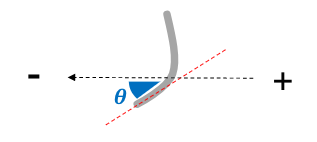
\includegraphics[width=0.6\textwidth]{../Figures/angle.png}
	\caption{How the angle in reponse to the EF is measured: The angle \( \Theta \) represents the angle between the line through the tip of the root and the point of highest local curvature and a line parallel to the EF; taken from [INSERT REFERENCE].}
	\label{fig:angle}
\end{figure}



Once these two lines are correctly defined, provided the point of highest local curvature is unique, it is straight forward to compute angle \( \Theta \).


%There are other ways such as finding vectors on the lines and using their dot products. However, we can use simple, basic trigonometric methods as shown in figure [INSERT REFERENCE HERE].
%
%We would then compute the angles of the two lines to the x-axis  in radians mode by 
%\[
%\pi - | \tan^{-1}(\frac{x(2) - x(1)}{y(2) - y(1)}) - \tan^{-1}(\frac{z(2) - z(1)}{y(2) - y(1)}) |
%\]
%or 
%\[
%180^{\circ} - | \tan^{-1}(\frac{x(2) - x(1)}{y(2) - y(1)}) - \tan^{-1}(\frac{z(2) - z(1)}{y(2) - y(1)}) |
%\]
%if we wanted it in degrees mode.
%
%The single steps are shown in figure ....
%[PSEUDOCODE]
%\begin{enumerate}
%	\item Find the slope of each line.
%	\item Find the inclination of each line using \( \alpha = \tan^{-1} m \), where  \( \alpha \) is the angle of inclination, \( m \) is the slope.
%	\item Take the difference of these two angles.
%	\item Handle the case where this difference is not an acute, i.e. less than 90 degrees, angle. If we get a negative angle, we take its absolute value. We want to find an acute angle, so if we calculated an obtuse angle, oe greater than 90 degrees, we just subtract the value from pi radians or 180 degrees to get the acute values.
%\end{enumerate}


%We refer to figure [INSERT REFERENCE HERE] to how the angle was computed in previous approaches. 


Let \( v_{1} \) be the line through the tip of the root and the point of highest local curvature and \( v_{2} \) a line parallel to the EF. 
We can compute angle \( \Theta \)  by using simple trigonometric methods 

\begin{equation} \label{angle1}
\Theta_{1}  = \cos^{-1}\frac{( v_{1} \cdot v_{2}) }{ | v_{1} | \cdot | v_{2} |}
\end{equation}
or equivalently
\begin{equation} \label{angle2}
\Theta_{2} = \tan^{-1}( v_{1}, v_{2}) \times \frac{180}{\pi}
\end{equation}
depending on the signedness of \( v_{1} \) and \( v_{2} \). Assuming the tip of the root only bends positively, i.e. towards the cathode (the negative pole of the EF) in our experimental setup, and \( v_{2} \) is not positive nor negative, the sign of \( \Theta \) only depends on \( v_{1} \). If the root tip crosses the line that is completely aligned with, i.e. parallel to, the EF (where \( \Theta \) takes the value 0), \( \Theta \) becomes negative as \( v_{1} \) will become negative. 


%----------------------------------------------------------------------------------------
\subsection{Computing the curvature of the root tip}


In order to detect the point of highest local curvature, we need to compute the curvature at each point in the skeleton. 


In the following, we will sketch the mathematical framework which describes the curvature of a curve embedded in a plane.
%For that, we want to introduce the reader to the concepts of a mathematical curvature in order 
This will help the user to understand the rather formula intense implementation computing the analytical curvature using fitted polygons to the points, i.e. the coordinates from the root skeleton.

There exist various different concepts and definitions of curvature in different branches of geometry.
Intuitively, curvature in the 2D case captures the amount by which a curve deviates from being a (straight) line.
We will only touch upon \textit{extrinsic} curvature here, which is defined for objects embedded in some higher-dimensional usually Euclidean space. This allows us to use the radius of circles that touch the object, so-called \textit{osculating cirlces}, to compute the curvature.

% Curvature is usually a scalar quantity, but one may define a curvature vector that takes into account the direction of the bend in addition to its magnitude.
% The curvature of more complex objects (such as surfaces or even curved n-dimensional spaces) is described by more complex objects from linear algebra, such as the general Riemann curvature tensor. 

Geometrically, the curvature measures how fast the unit tangent vector, i.e. the vector tangent to the curve and of length 1,  to the curve rotates. 
[INSERT FIGURE HERE]

If the curve is close to a straight line, and thus the unit tangent vector changes very little, the curvature is small; if the curve contains a sharp turn, the curvature is large.
In the implementations we used the difference between edge direction vectors to compute this velocity.


%INSERT PRECISE DEFINITION HERE AND INSERT HERE "CURVATURE OF SPACE CURVES" FROM WIKIPEDIA


%For the implementation 
We first compute the first derivative (in between pairs of samples), and we take into account unequal segment lengths. In the same way we then compute the second derivative, we take the average length of two neighbouring edges, i.e. the length of edge in between neighbouring normals if we consider the normals to be halfway between vertices.
Once we have the normals, we can compute the rate of change between neighbouring normals to assign the specific curvature value to each point.

[INSERT FIGURE HERE, DRAW IT]

%The current implementation of the \textit{getAngle.m} script fits polygons to the points, i.e. the coordinates from the root skeleton, and then calculates the analytical curvature from these fitted polygons. 

If the user does not specify otherwise, we assume the line pieces to connect two neighbouring points. The curvature function outputs a vector of curvature values of the points.


%I wish to calculate the curvature (as accurate as possible) at the points on the curve.
% what I have until now is a simple calculation of the tangent vector (1st derivate) and then the curvature (2nd derivate):


In a previous version, we  took a section of the curve (here 9 vertices) and fitted a polynomial to it; this will be our cuve model. From this model we can compute the derivative and with the coefficients of the fitted polynomial we can compute the curvature at each point. 
A large radius of the osculating circle, i.e. a high curvature, means a rather straight part of the curve, while we get a small radius or curvature in parts where the curve is "pointy", i.e. bends more. The sign of the curvature indicates whether it is right (positive) or left (negative) bending. However, the here used function \textit{polyfit} should not be used on very noisy data.



%REFERENCES:  Rusinkiewicz, "Estimating Curvatures and Their Derivatives on Triangle Meshes
%gfx.cs.princeton.edu/pubs/_2004_ECA/curvpaper.pdf
%https://www.google.com/url?sa=t&rct=j&q=&esrc=s&source=web&cd=4&ved=2ahUKEwijgv644IvdAhUHTsAKHfYiAVQQFjADegQIBxAC&url=http%3A%2F%2Fwww.cs.jhu.edu%2F~misha%2FFall09%2F4-surfaces.pdf&usg=AOvVaw2wHCpX0Ruh46CviayKYl0d

%http://http.cs.berkeley.edu/~jrs/meshpapers/MeyerDesbrunSchroderBarr.pdf

%REFERENCES: https://www.jstor.org/stable/10.4169/amer.math.monthly.122.04.332?seq=1#page_scan_tab_contents


%%%%%%%%%%%%%%%%%%%%%%%%%%%%%%%%%%%%%%%%%%%%

%
%  k = LineCurvature(Vertices,Lines)
% 
% inputs,
%   Vertices : A M x 2 list of line points.
%   (optional)
%   Lines : A N x 2 list of line pieces, by indices of the vertices
%         (if not set assume Lines=[1 2; 2 3 ; ... ; M-1 M])
%
% outputs,
%   k : M x 1 Curvature values
%
% If no line-indices, assume a x(1) connected with x(2), x(3) with x(4)


% Fit polygons to the vertices 
% x=a(3)*t^2 + a(2)*t + a(1) 
% y=b(3)*t^2 + b(2)*t + b(1) 
% we know the x,y of every vertex and set t=0 for the vertices, and
% t=Ta for left vertices, and t=Tb for right vertices,  


%APPROACH 1
% Use skeleton/bwboundaries to get a list of the (x,y) boundary coordinates. 
% Run around that border taking a section of the curve, say 9 elements, and fit 
% a polynomial to it. Knowing the derivative of the curve model I used, and 
% the coefficients polyfit() gave me, I can get the curvature at each point. 
% [Optional: Then I run around the list of (x,y) edge coordinates using a marker color 
% that corresponds to the curvature.]

% A large radius of curvature means a "flat" part of the curve while a small radius 
% of curvature means "pointy" parts of the curve.
% Whether it is positive or negative just says which side of the curve it is bending to. 
% I could just take the absolute value of the curvature if I do not care which 
% side it bends toward; however, we do care as the root bends positively (clockwise).


%OLD APPROACHES:

%CURVATURE VIA TRIANGLE -- 3 POINTS 

%ANGLE BETWEEN TWO POINTS USING SCALAR PRODUCT
 
%CURVATURE USING FORMULA FROM PAPER ROBERT ISRAEL



%%----------------------------------------------------------------------------------------
%\subsection{Using the position of the tip of the root -- more in detail}
%
%INSERT FIGURE OF WHAT ANGLE WE CALCULATE AND WHAT IS THE ANGLE OF INTEREST. 
%USER-FRIENDLY: EASILY SWITCH BETWEEN THE TWO OF THEM.
%
%We find the angle between the two lines (point of highest mean curvture OR manually click point of highest curvature and tip and point of highest mean curvature and equally distant point/ pixel on root).


%
%%----------------------------------------------------------------------------------------
%\subsection{Using the angle of the tangents to the points that are x points/pixels away from the point of highest local curvature}
%
%%\subsection{INSERT VARIOUS OTHER IDEAS OF ANGLE COMPUTATION -- even if not implemented}
